\section{Analisi e Conclusioni}

\subsection{Controllo dei falsi allarmi}
La correttezza dell'implementazione di un test di ipotesi può essere controllata assicurandosi che in condizioni di ipotesi nulla il test produca esattamente $\alpha$\% falsi allarmi. Il test deve poi presentare la maggiore potenza possibile in caso di ipotesi contraria. Per utilizzare una metrica di riferimento abbiamo utilizzato i test inclusi nella libreria standard di matlab.
Mostriamo quindi il risultati ottenuti dall'uso di una semplice statistica, la differenza delle medie:

\begin{center}
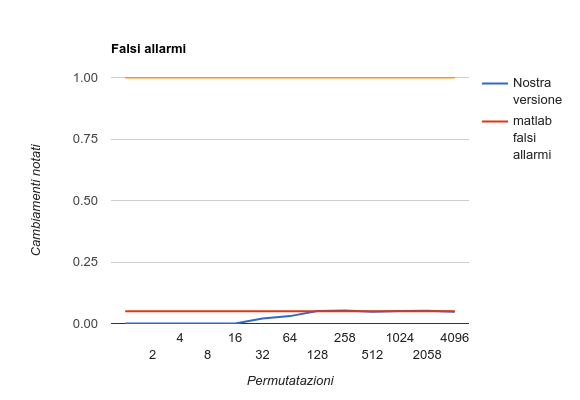
\includegraphics[width=\linewidth]{falsi_allarmi}
\captionof{figure}{Falsi allarmi}
\end{center}

La linea rossa è generata da matlab non dipende dal numero di permutazioni, quindi è costante a 0.05, come ci si attende. La linea blu rappresenta invece la nostra versione del permutation test, la quale per bassi valori di permutazione è del tutto incapace di notare cambiamenti nei valori in ingresso. Quando le permutazioni aumentano i falsi allarmi si stabilizzano velocemente ad $\alpha$. 

Ora che siamo certi che sotto ipotesi nulla il nostro algoritmo si comporta correttamente, possiamo quindi analizzare il caso in cui i gruppi provengono da popolazioni diverse.
\begin{center}
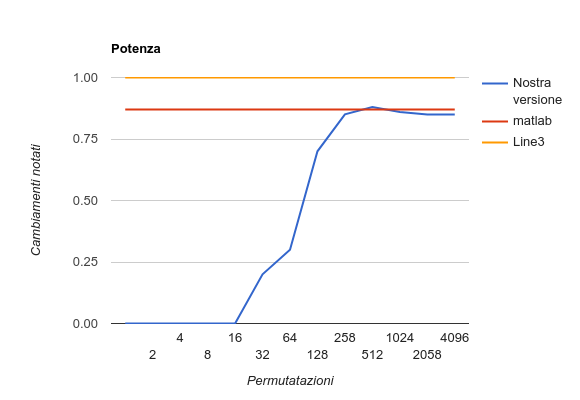
\includegraphics[width=\linewidth]{potenza}
\captionof{figure}{Potenza test}
\end{center}

Come nel caso precedente si nota che pur fallendo per permutazioni in quantità minute risulta che il test produce risultati simili a quello standard. Si noti inoltre che come nel caso precedente non sembra esserci alcun vantaggio nell'utilizzare un grande numero di permutazioni, poiché quando raggiungono l'ordine delle centinaia la potenza si stabilizza. Questo significa che, date le ottimizzazioni sull'uso della memoria, se si fissa un numero di permutazioni, è possibile processare set di dati con utilizzi di tempo e memoria che dipendono linearmente solo dalla dimensione dei dati in ingresso. Poiché è evidente che per processare un set di dati è per lo meno necessario valutare almeno una volta tutti gli elementi, ciò risulta essere il migliore risultato possibile. 

Ciò che rimane è mostrare la velocità di throughput che è possibile raggiungere è superiore ad un implementazione basata su cpu.

\subsection{Benchmark}
\begin{center}
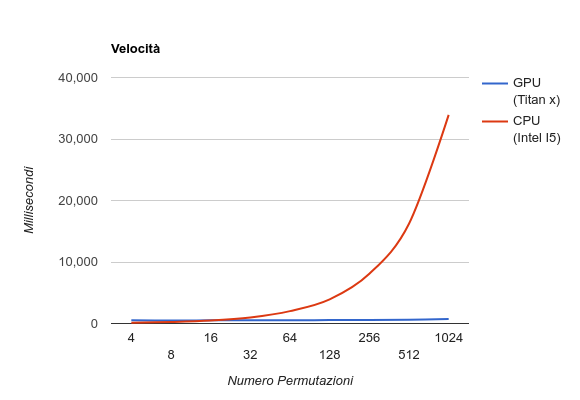
\includegraphics[width=\linewidth]{confronto}
\captionof{figure}{Confronto GPU vs CPU}
\end{center}
Il tempo necessario al completamento del calcolo dell'implementazione su cpu dipende linearmente dalla quantità di permutazioni, e allo spostarsi verso destra sull'asse X diventa rapidamente troppo lento. La implementazione GPU invece sembra rimanere a tempo costante, ciò è dovuto al fatto che le permutazioni non superano in quantità il numero di core a disposizione sulla scheda e quindi tutti il calcoli possono avvenire allo stesso momento. 
Come ci si aspettava l'implementazione su GPU risulta essere meno performante per piccoli valori di permutazioni, dove i vantaggi dell'architettura parallela sono ridotti, ma non appena si supera una soglia critica la implementazione su gpu risulta più efficiente sotto tutti gli aspetti.

Studiano più accuratamente solo i risultati della gpu risulta inoltre:

\begin{center}
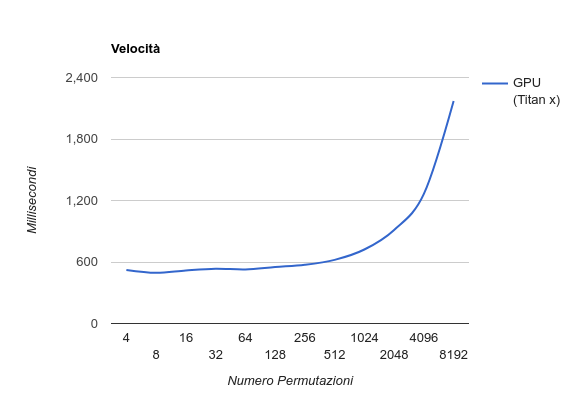
\includegraphics[width=\linewidth]{analisi}
\captionof{figure}{Velocità GPU nel dettaglio}
\end{center}
Per piccoli valori di permutazioni il tempo richiesto è effettivamente costante, mentre esso ritorna a dipendere linearmente dal numero di permutazioni non appena la scheda viene saturata.
Anche in questo caso il tempo per impiegare 8192 permutazioni è circa 2.5, inferiore a quello necessario per compierne 512 su una cpu. Si noti inoltre che non si erano trovati significativi incrementi di potenza quando il numero di permutazioni superava l'ordine delle centinaia, di conseguenza non vi è motivo di operare nello spazio in cui il tempo di esecuzione dipende linearmente dal numero di permutazioni. Ciò trasforma la nostra implementazione in un algoritmo che opera a tempo costante su set di dati di dimensione fissata dotato di potenza simile a quella dei test disponibili nelle librerie standard ma con un througthput maggiore e capace di operare su dati multivariati, il che era l'obiettivo che si intendeva raggiungere in questo documento.

Le ottimizzazioni inoltre producono i seguenti incrementi in performance:

\begin{center}
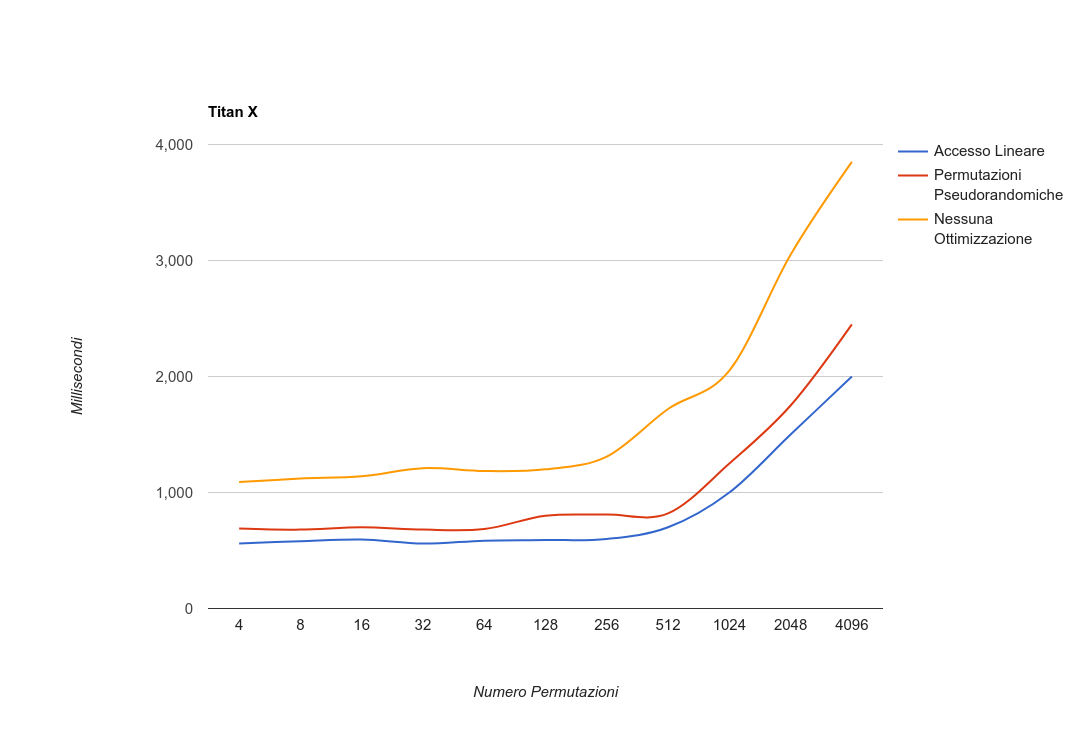
\includegraphics[width=\linewidth]{ott}
\captionof{figure}{Confronto ottimizzazioni}
\end{center}
La linea blu rappresenta l'implementazione OpenCL triviale, come ci si aspetta risulta essere due volte peggiore che la implementazione ottimizzata. La linea rossa rappresenta invece la versione dell'algoritmo dotata di permutazione pseudorandomica ma di cui non è garantito l'accesso ordinato alla memoria. In questo caso ne prestazioni sono paragonabili alle migliori rilevate, sebbene una diminuzione del tempo di calcolo di un sesto giustifica l'uso di codice più complesso e difficile da mantenere.

\subsection{Lavori Futuri}
A seconda di quale sia il campo di applicazione di un test di ipotesi ad alta velocità è possibile che ulteriori caratteristiche oltre a quelle indicare siano richieste. Si può immaginare che la necessità di analizzare eventi che avvengono ad alta frequenza sia spesso associata alla necessità di processare tali dati sotto forma di stream continui fino a che non viene notato un cambiamento nella natura dei dati osservati.
Una delle soluzioni di tale problema prende il nome di Change Point Model (CPM) e consiste nell'analizzare i dati per ogni possibile posizione del change point, per poi selezionare la posizione che più si è discostata dalla soglia. Il tentativo di integrare il permutation test e il CPM si è rivelato più complesso del prevsito, le integrazioni più semplici sono inefficienti, poiché le ottimizzazioni necessarie ad uno risultano in un peggioramento delle prestazioni dell'altro. Questo limite pare significativo e ne consegue che la risoluzione possa essere soggetto di ulteriori studi.